\section{Overview}
\begin{frame}{Nonlinear Invariant Attack}{Practical Attack on Full SCREAM, iSCREAM, and Midori64}
    \begin{block}{Paper}
        \begin{itemize}
            \item \textcite{AC16:TLS} at AsiaCrypt'16
            \item Structural attack, brakes SCREAM, iSCREAM and Midori64
                  (surprise, surprise)\footnote{Useless \LaTeX{} Fact: Did you know that \texttt{\textbackslash{}time} is an anagram of \texttt{\textbackslash{}item}?}
                  in the \emph{weak key setting}
        \end{itemize}
    \end{block}
    \begin{columns}[T]
        \begin{column}{0.45\textwidth}
            \begin{block}{Organisation}
                \vspace{0.5em}
                \tableofcontents
            \end{block}
        \end{column}
        \begin{column}{0.45\textwidth}
        \end{column}
    \end{columns}
\end{frame}

\section{The Context}
\begin{frame}{Context}{or: similar attacks?}
    \begin{block}{Attacks in Symmetric Cryptanalysis}
        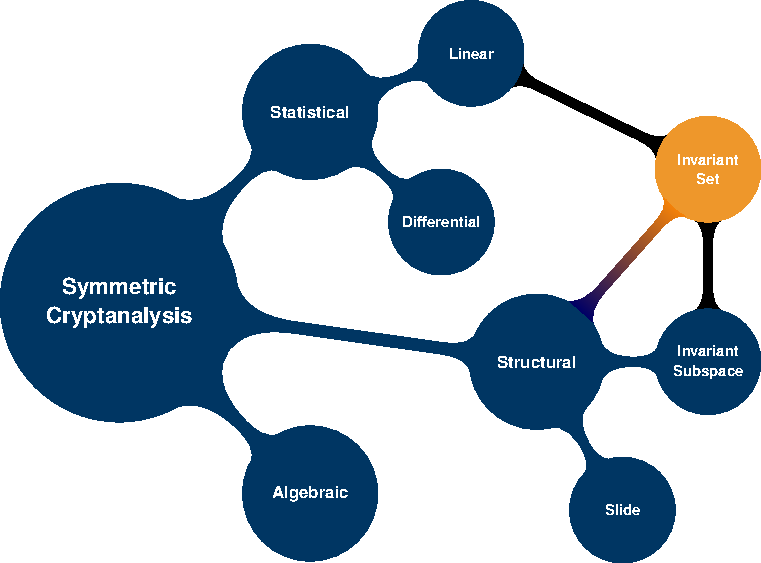
\includegraphics[keepaspectratio, height=0.7\textheight]{data/mindmap}
    \end{block}
\end{frame}

\begin{frame}{Linear Cryptanalysis}{Taking the fun out of it}
    \only<1>{%
        \begin{columns}[T]
            \begin{column}{.58\textwidth}
                \begin{itemize}
                    \item invented by \textcite{EC93:Mat}
                    \item broke DES
                    \item together with Differential Cryptanalysis best studied attack on block ciphers
                \end{itemize}
            \end{column}
            \hfill
            \begin{column}{.38\textwidth}
                \begin{figure}[!ht]
                    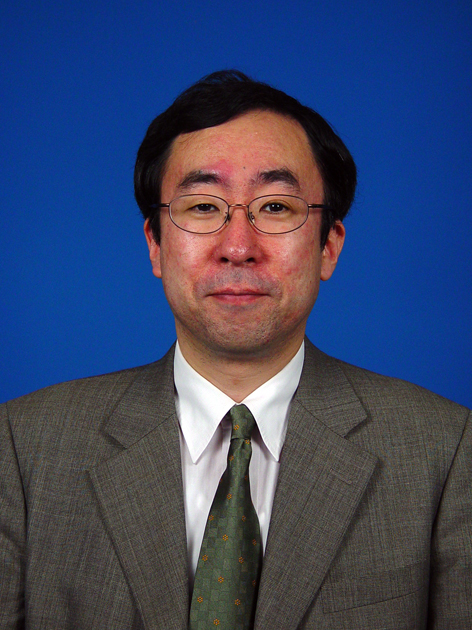
\includegraphics[height=50mm]{data/matsui.jpg}
                \end{figure}
            \end{column}
        \end{columns}\blfootnote{\scriptsize Image: \url{http://www.isce2009.ryukoku.ac.jp/eng/keynote_address.html}}
    }
    \only<2->{%
        \begin{block}{Core Idea}
            Given a block cipher $E_k : \F_2^n \to \F_2^n$, find an \emph{input mask} $\alpha \in \F_2^n$ and an \emph{output mask} $\beta \in \F_2^n$, \st/
            \begin{equation*}
                \angles{\alpha, x} \oplus \angles{\beta, E_k(x)} = c
            \end{equation*}
            holds with high probability for a constant $c$.
        \end{block}
        \begin{itemize}
            \item $\alpha \stackrel{E_k}{\longrightarrow} \beta$ is called a \emph{linear approximation} of $E_k$
            \item much more to deal with: we have to keep the distribution over $k$ in mind and so on and so forth
        \end{itemize}
    }
\end{frame}

\begin{frame}{Invariant Subspace Attack}{Almost there}
    \only<1>{%
        \begin{columns}[T]
            \begin{column}{.58\textwidth}
                \begin{itemize}
                    \item invented by \textcite{C:LAAZ11}
                    \item broke \textsc{PRINTcipher}
                \end{itemize}
            \end{column}
            \hfill
            \begin{column}{.38\textwidth}
                \begin{figure}[!ht]
                    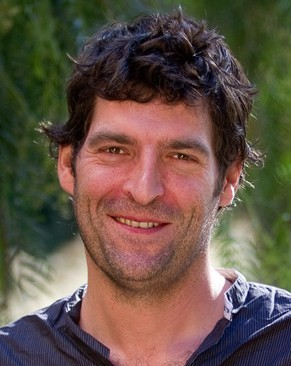
\includegraphics[height=50mm]{data/leander.jpg}
                \end{figure}
            \end{column}
        \end{columns}\blfootnote{\scriptsize Image: \url{http://www.lightsec.org/2013/images/gregor_leander.jpg}}
    }
    \only<2->{%
        \begin{block}{Core Idea}
        \end{block}
        \begin{itemize}
            \item \ldots
        \end{itemize}
    }
\end{frame}

\section{The Attack}
\begin{frame}{Invariant Set Attack}{or: Nonlinear Invariant Attack}
    \begin{block}{Core Idea}
        Given a block cipher $E_k : \F_2^n \to \F_2^n$, \st/ $E_k(x) = E(x \oplus k)$, find an efficiently computable nonlinear Boolean function $g : \F_2^n \to \F_2$, \st/
        \begin{equation}
            g(E(x \oplus k)) = g(x \oplus k) \oplus c = g(x) \oplus g(k) \oplus c
            \label{eq:g}
        \end{equation}
        for a constant $c$ and many $k$.
    \end{block}
    \begin{itemize}
        \item $g$ is called \emph{nonlinear invariant}
        \item keys for which Eq~\eqref{eq:g} holds are called \emph{weak keys}
    \end{itemize}
\end{frame}

\begin{frame}{Invariant Set Attack}{Step-by-Step}
    \only<1>{%
        \begin{block}{Typical block cipher construction: key-alternating function}
            Let $F :  \F_2^n \to \F_2^n$ and $E_{k_1, k_2, \ldots, k_r} : \F_2^n \to \F_2^n$ be of the form
            \begin{equation*}
                E_k(x) = F( \cdots F(x \oplus k_1) \cdots \oplus k_{r}).
            \end{equation*}
        \end{block}
    }
    \visible<2->{%
        Notation: we write $y_0 = x$, $y_i = F(y_{i-1} \oplus k_i)$, and thus $y_r = E_k(x)$.
        \begin{block}{Nonlinear invariant for the round function}
            Assume there exists a nonlinear invariant $g$ for $F$, \st/ all keys $k_i$ are weak.
            Then:
            \visible<3->{%
                \begin{align*}
                    g(E_k(x)) &= g(y_r) \\
                    \visible<4->{&= g(F(y_{r-1} \oplus k_r)) \\}
                    \visible<5->{&= g(y_{r-1}) \oplus g(k_r) \oplus c_r\\}
                    \visible<6->{&\hspace{0.625em}\vdots \\[-0.75em]
                                 &= g(x) \oplus \bigoplus_{i=1}^r g(k_i) \oplus c_1}
                \end{align*}
            }
        \end{block}
    }
\end{frame}

\begin{frame}{Invariant Set Attack}{Weak Keys}
    It seems quite unlikely that Eq~\eqref{eq:g} holds for many $k$.
    \begin{block}{Example nonlinear invariant}
        \vspace{-2em}
        \begin{align*}
            g : \F_2^4 &\to \F_2 \\
            (x_4, x_3, x_2, x_1) &\mapsto x_4 x_3 \oplus x_3 \oplus x_2 \oplus x_1
        \end{align*}
        \vspace{-2em}
    \end{block}
    \visible<2->{%
        \begin{exampleblock}{$g$ is nonlinear invariant for key xor and has 4 weak keys:}
            Split $g$ in a nonlinear part $f$ and a linear part $\ell$:
            \begin{equation*}
                g(x_4, x_3, x_2, x_1) = f(x_4, x_3) \oplus \ell(x_2, x_1)
            \end{equation*}
            All $k$ of the form $k = (0, 0, k_2, k_1)$ are weak -- and these are exactly four possible keys.
        \end{exampleblock}
    }
\end{frame}

\section{The Results}
\begin{frame}{Results}{}
    \begin{block}{Attack Complexities}
        \centering
        \begin{tabular}{ccc}
            \toprule
                   & \# Weak $k$ & max. \# Recovered Bits \\
            \midrule
             SCREAM &  $2^{96} $  &       $32$~bits  \\
            iSCREAM &  $2^{96} $  &       $32$~bits  \\
           Midori64 &  $2^{64} $  &      $32h$~bits  \\
            \bottomrule
        \end{tabular}

        \begin{tabular}{ccc}
            \toprule
                   & Data Complexity & Time Complexity \\
            \midrule
             SCREAM &  $33$~ciphertexts  & $32^3$  \\
            iSCREAM &  $33$~ciphertexts  & $32^3$  \\
           Midori64 &  $33h$~ciphertexts & $32^3 \cdot h$  \\
            \bottomrule
        \end{tabular}
    \end{block}
\end{frame}
